\documentclass[a4paper, 12pt]{article}
\usepackage[hmargin=2cm,vmargin=2.5cm]{geometry}
\usepackage[polish]{babel}



\usepackage{listings}
\usepackage{color}
% Define Gruvbox colors
\definecolor{gruvbox-bg}{rgb}{0.156,0.156, 0.156}
\definecolor{gruvbox-fg}{rgb}{0.92 , 0.85, 0.69}
\definecolor{gruvbox-comment}{rgb}{0.57, 0.51, 0.45}
\definecolor{gruvbox-purple}{rgb}{0.82, 0.52, 0.60}
\definecolor{gruvbox-green}{rgb}{0.72, 0.72, 0.14}

% Define the lstlisting style using Gruvbox colors
\lstdefinestyle{mystyle}{
    language=Python,
    backgroundcolor=\color{gruvbox-bg},   
    basicstyle=\color{gruvbox-fg}\ttfamily\scriptsize,
    commentstyle=\color{gruvbox-comment},
    keywordstyle=\color{gruvbox-purple},
    stringstyle=\color{gruvbox-green},
    numberstyle=\tiny\color{gruvbox-comment},
    breakatwhitespace=false,         
    breaklines=true,                 
    captionpos=b,                    
    keepspaces=true,                 
    numbers=left,                    
    numbersep=5pt,                  
    showspaces=false,                
    showstringspaces=false,
    showtabs=false,                  
    tabsize=2
}

\lstset{style=mystyle}


\usepackage{float}
\usepackage{enumerate}
\usepackage{makecell}
\usepackage{graphicx}
\usepackage{hyperref}
\usepackage{amsmath}
\usepackage[table]{xcolor}
\usepackage{tabularray}
\usepackage{csquotes}

\usepackage[T1]{fontenc}


\setlength{\arrayrulewidth}{0.4mm}

\newcommand{\HRule}{\rule{\linewidth}{0.5mm}}


\usepackage{enumitem}

\begin{document}

\begin{titlepage}
  \begin{center}
    % logo
    
\includegraphics[width=0.5\textwidth]{images/logo.png}~\\[1cm]

    \textsc{Sprawozdanie z zajęć laboratoryjnych\\ Sztuczna inteligencja i inżynieria wiedzy\\[3cm]}


    \HRule \\[0.4cm]
    {\large \bfseries Lista 01 \\ Problemy optymalizacyjne i algorytmy przeszukiwania\\[0.4cm]}
    \HRule \\[8cm]


    Tomasz Mroczko, 266604 \\[3cm]

    \vfill

    {\today}

  \end{center}
\end{titlepage}


\newpage
\tableofcontents
\newpage


\section{Dane}

  \subsection{Zawartość}
  Dane zawarte w pliku \textit{connection\_graph.csv} zawierały informacje o połączeniach komunikacyjnych
  pomiędzy przystankami komunikacji miejskiej we Wrocławiu. Każdy wiersz zawiera informacje o połączniu pomiędzy dwoma przystankami w postaci:
  \begin{itemize}
    \item id - identyfikator połączenia
    \item company - przewoźnik
    \item line - numer linii
    \item departure\_time - czas odjazdu w formacie HH:MM:SS
    \item arrival\_time - czas przyjazdu w formacie HH:MM:SS
    \item start\_stop - nazwa przystanku początkowego
    \item end\_stop - nazwa przystanku końcowego
    \item start\_stop\_lat - szerokość geograficzna przystanku początkowego
    \item end\_stop\_lat - szerokość geograficzna przystanku końcowego
    \item start\_stop\_lon - długość geograficzna przystanku początkowego
    \item end\_stop\_lon - długość geograficzna przystanku końcowego
  \end{itemize}
  Rozmiar pliku wynosił 113MB, i zawierał on 996 521 wierszy.


  \subsection{Wstepna analiza}
    Pierwotna analiza danych, wykazała, że w pliku znajduje się bardzo dużo 
    powtarzających się wierszy, które różnią się jedynie id. Sugeruje to, że dane zostały sztucznie "wydłużone",
    prawdopodobnie w celu jaśniejszego zaznaczenia różnicy pomiędzy szybkością działania algorytmów poprzez wydłużenie
    czasu przeszukiwania. Jednak jest to tylko domysł, a nie potwierdzona informacja.  \\

    \begin{lstlisting}[language=bash]
      cat connection_graph.csv | cut -d',' -f2- | sort | uniq | wc -l
    \end{lstlisting}

    Za pomocą tej komendy, sprawdzono unikalność wierszy w pliku. Znaczna część wierszy jest duplikatami.
    Ustalono, że jedynie 455 232 wieszy jest unikalnych (mniej niż połowa).
    Pomimo tego faktu, do dalszej analizy użyto pełnego pliku, bez usuwania duplikatów. \\
    Warto zaznaczyć, że godziny odjazdu po 23:59:59 były zapisywane jako 24:00:00, co jest niepoprawne w kontekście
    zapisu czasu w formacie 24-godzinnym. Ponieważ przyjęto reprezentację odjazdju jako liczba minut od północy,
    nie było to problemem w dalszej analizie. \\

  \subsection{Reprezentacja}
    Dane reprezentowane są za pomocą kilku struktur danych w celu ułatwienia organizacji i przetwarzania.
    Dla przystanku oraz połączenia użyto NamedTuple zamiast klasy, ze względu na prostotę, niemutowalność
    i szybkość działania. Takie podejście pozwoliło uzyskać namiastkę typowania poprzez adnotacje typów
    w Pythonie, co ułatwiło pisanie kodu, a także pozwoliło \href{https://microsoft.github.io/language-server-protocol/}{\color{gruvbox-purple}LSP}
    na podpowiadanie nazw pól oraz analizowanie kodu.

    \begin{itemize}
      \item \textbf{Stop} - reprezentuje pojedynczy przystanek. 
        Przystanek jest reprezentowany przez nazwę, szerokość i długość geograficzną,
        jednak do porównywania przystanków używane jest jedynie pole z nazwą. Identyfikowanie ich także poprzez
        długość i szerokość geograficzną powodowało duże problemy związane z przeszukiwaniem połączeń (kierunki odjazdów,
        przystanki autobusowe a tramwajowe, wprowadzanie nazw przystanków, itp.).
        \begin{lstlisting}[language=Python]
class Stop(NamedTuple):
    name: str
    lat: float
    lon: float

    def __eq__(self, other: object) -> bool:
        if not isinstance(other, Stop):
            return False
        return self.name == other.name

    def __hash__(self) -> int:
        return hash(self.name)

    def __repr__(self) -> str:
        return f"Stop: {self.name}"
        \end{lstlisting}



      \item \textbf{Route} - reprezentuje połączenie miedzy przystankami. Ze względu na wydajność
      oraz prostotę obliczeń, czas odjazdu oraz przyjazdu został przekształcony na minutę od północy.
\begin{lstlisting}
class Route(NamedTuple):
    line: str
    start_stop: Stop
    end_stop: Stop
    departure_min: int
    arrival_min: int
    start_stop_lat: float
    start_stop_lon: float
    end_stop_lat: float
    end_stop_lon: float

    def __eq__(self, other) -> bool:
        if not isinstance(other, Route):
            return False
        return self.line == other.line and self.end_stop == other.end_stop

    def __hash__(self) -> int:
        return hash((self.line, self.end_stop.name))

    def __repr__(self) -> str:
        return f"{self.start_stop} -> {self.end_stop}: {self.departure_min}"
\end{lstlisting}

      \item \textbf{Graph} - klasa która agreguje przystanki oraz połączenia z nich odjeżdżające. 
      Posiada także zbiór unikatowych nazw linii, które przyjeżdżają na dany przystanek, używany
      w celu ulepszenia przseszukiwania pod kątem ilości przesiadek.
      
\begin{lstlisting}
class Graph:
    def __init__(self):
        self.departures: dict[Stop, list[Route]] = {}
        self.arriving_line_names: dict[Stop, set[str]] = {}

    def add_route(self, route: Route):
        if route.start_stop not in self.departures:
            self.departures[route.start_stop] = []
            self.arriving_line_names[route.start_stop] = set()

        if route.end_stop not in self.departures:
            self.departures[route.end_stop] = []
            self.arriving_line_names[route.end_stop] = set()

        self.departures[route.start_stop].append(route)
        self.arriving_line_names[route.end_stop].add(route.line)

    def get_stop(self, name: str) -> Optional[Stop]:
        for stop in self.departures:
            if stop.name == name:
                return stop
        return None

    def is_direct_connection(self, route: Route, destination: Stop) -> bool:
        return route.line in self.arriving_line_names[destination]
\end{lstlisting}


    \end{itemize}



\section{Zadanie 1}
  \subsection{a) Dijkstra - kryterium czasu}
  \subsubsection{Opis} Celem było zaimplementowanie algorytmu dijkstry, który
  znajduje najkrótszą ścieżkę pomiędzy dwoma przystankami, biorąc pod uwagę \textit{jedynie}
  czas podróży. 

  \subsubsection{Działanie / kod} Algorytm działa na zasadzie zachłannego przeszukiwania grafu w głąb.
  W każdym kroku wybierany jest wierzchołek, który ma najkrótszą odległość od źródła.
  Relizowane to jest za pomocą kolejki priorytetowej,
  która pozwala na wybieranie wierzchołka o najmniejszej wartości funkcji kosztu.  \\
  Dla każdej krawędzi liczona jest liczba minut potrzebna na przejazd do danego przystanku.
  Jeśli odległość ta jest mniejsza niż dotychczasowa, to aktualizowana jest odległość oraz poprzednik,
  który pozwoli na odtworzenie ścieżki, a następnie wierzchołek dodawany jest do kolejki priorytetowej.
  Algorytm kończy się gdy dotrzemy do celu lub gdy kolejka priorytetowa jest pusta. \\
  \begin{itemize}
    \item Dijkstra
\begin{lstlisting}
@route_info_decorator
def dijkstra(graph: Graph, start: Stop, end: Stop, departure_min: int) -> SearchResult:
    costs: dict[Stop, float] = {start: 0}
    came_from: dict[Stop, Optional[Route]] = {start: None}

    pq: PriorityQueue[tuple[float, Stop]] = PriorityQueue()
    pq.put((0, start))

    visited_stops_counter: int = 0
    while not pq.empty():
        visited_stops_counter += 1
        curr_cost, curr_stop = pq.get()
        prev_route: Optional[Route] = came_from[curr_stop]

        if curr_stop == end:
            break

        for route in graph.departures[curr_stop]:
            end_stop: Stop = route.end_stop
            route_cost = curr_cost + minutes_cost(
                prev_route, route, int(departure_min + curr_cost)
            )

            if end_stop not in costs or route_cost < costs[end_stop]:
                costs[end_stop] = route_cost
                came_from[end_stop] = route
                pq.put((route_cost, end_stop))

    return SearchResult(costs, came_from, end, visited_stops_counter)
\end{lstlisting}
  Dodatkowo, algorytm jest ozdobiony dekoratorem, który zajmuje się 
  przeanalizowaniem oraz wypisaniem informacji o jego przebiegu.
  Algorytm zwraca strukturę SearchResult,
  która zawiera informcje o kosztach, poprzednikach oraz liczbę odwiedzonych przystanków.
  \item SearchResult
\begin{lstlisting}
class SearchResult(NamedTuple):
    costs: dict[Stop, float]
    came_from: dict[Stop, Optional[Route]]
    end_stop: Stop
    visited_stops: int
\end{lstlisting}

  \item minutes\_cost
\begin{lstlisting}
def minutes_cost(
    prev_route: Optional[Route], curr_route: Route, curr_minutes: int
) -> int:
    MINUTES_IN_DAY: int = 24 * 60
    delay = 0

    if prev_route is None or prev_route.line == curr_route.line:
        if curr_minutes > curr_route.departure_min:
            delay = MINUTES_IN_DAY
    elif prev_route.line != curr_route.line:  # there is a line change
        # modify this to take more time for change
        if curr_minutes > curr_route.departure_min:
            delay = MINUTES_IN_DAY
    return curr_route.arrival_min + delay - curr_minutes
\end{lstlisting} 
  Funkcja oblicza czas przejazdu pomiędzy dwoma przystankami. 
  Jeśli jest to przesiadka, to wymagany może być dodatkowy czas na zmianę linii.



  \end{itemize}
  






  \subsubsection{Wnioski} Algorytm Dijkstry biorący pod uwagę czas podróży działa poprawnie.
  W tym wypadku zachłanność algorytmu nie powinna stanowić problemu, poniweaż 
  optymalizacja czasu dojazdu lokalnie jest jednoznaczna, i nie powinna uniemożliwić dotarcia do celu 
  optymalną trasą (zawsze możemy przesiąść się do optymalnej linii).

  \subsection{b) A* - kryterium czasu}

  \subsubsection{Opis}
  Algorytm ten jest rozszszeniem algorytmu Dijkstry, który w celu szybszego znalezienia 
  ścieżki. Różni się on jedynie uwzględnieniem w priorytecie kolejki dodatkowej heurystyki,
  która jest oszacowaniem odległości od danego wierzchołka do celu. Dzięki temu, najpierw analizowane 
  są wierzchołki, które mają najmniejszą wartość heurestyki oraz funkcji celu.
  Heurestyka to zazwyczaj odległość mierzona pomiędzy dwoma punktami. W tym przypadku,
  heurestyka jest wstrzyknięta do algorytmu, co pozwala na łatwe zmienianie jej wartości.
  Używane przeze mnie heurestyki to odległość manhattan(pionowa + pozioma) oraz odległość haversine
  (odległość geograficzna w km).

  \subsubsection{Działanie / kod}
  Algorytm ten tak naprawdę różni się od Dijkstry jedynie w sposobie obliczania priorytetu w kolejce.
  W tym wypadku, priorytetem jest suma kosztu oraz heurestyki.
  \begin{itemize}
    \item A*
\begin{lstlisting}
def astar_time(
    graph: Graph,
    start: Stop,
    end: Stop,
    departure_min: int,
    heuristic: Callable[[Stop, Stop], float],
    heuristic_weight: float,
) -> SearchResult:
    costs: dict[Stop, float] = {start: 0}
    came_from: dict[Stop, Optional[Route]] = {start: None}

    pq: PriorityQueue[tuple[float, Stop]] = PriorityQueue()
    pq.put((0, start))

    visited_stops_counter: int = 0
    while not pq.empty():
        visited_stops_counter += 1
        _, curr_stop = pq.get()
        curr_cost = costs[curr_stop]
        prev_route: Optional[Route] = came_from[curr_stop]

        if curr_stop == end:
            break

        for route in graph.departures[curr_stop]:
            end_stop: Stop = route.end_stop
            route_cost = curr_cost + minutes_cost(
                prev_route, route, int(departure_min + curr_cost)
            )

            if end_stop not in costs or route_cost < costs[end_stop]:
                costs[end_stop] = route_cost
                came_from[end_stop] = route

                priority = route_cost + heuristic(end_stop, end) * heuristic_weight
                pq.put((priority, end_stop))

    return SearchResult(costs, came_from, end, visited_stops_counter)
\end{lstlisting}


\item Heurystyki
\begin{lstlisting}
def manhattan_distance(start: Stop, end: Stop) -> float:
    # usually something around 0.1 so scale it to about 1
    DISTANCE_SCALE = 10

    distance = abs(end.lat - start.lat) + abs(end.lon - start.lon)

    return distance * DISTANCE_SCALE


def haversine_distance(stop1: Stop, stop2: Stop) -> float:
    # usually around 5, so scale it down to about 1
    DISTANCE_SCALE = 1 / 5

    lat1_rad = math.radians(stop1.lat)
    lon1_rad = math.radians(stop1.lon)
    lat2_rad = math.radians(stop2.lat)
    lon2_rad = math.radians(stop2.lon)

    dlat = lat2_rad - lat1_rad
    dlon = lon2_rad - lon1_rad

    a = (
        math.sin(dlat / 2) ** 2
        + math.cos(lat1_rad) * math.cos(lat2_rad) * math.sin(dlon / 2) ** 2
    )

    c = 2 * math.atan2(math.sqrt(a), math.sqrt(1 - a))
    radius_of_earth_km = 6371.0
    distance_km = radius_of_earth_km * c

    return distance_km * DISTANCE_SCALE
\end{lstlisting}
  Heurestyki zostały skalowane w celu łatwiejszego wyważania ich wpływu na algorytm.
  Celem było uzyskanie wartości w okolicach 1, co pozwala na łatwe zmienianie wpływu heurestyki w
  dalszym działaniu.

\item Funkcja fabrykująca instancje algorytmu A* - ponieważ 
sygnatura funkcji jest inna niż algorytmu dijkstry, stworzono funkcję, która zwraca częściowo zaaplikowaną
funkcję, w celu ujednolicenia ich sygnatur, co pozwoli na łatwe przekazywanie ich do dekoratora i wywołanie.

\begin{lstlisting}
def create_astar(
    heuristic: Callable[[Stop, Stop], float], mode: str, print_result: bool = True
) -> Callable[[Graph, Stop, Stop, int], SearchResult]:

    if mode == "t":
        heuristic_weight: float = 30
    elif mode == "p":
        heuristic_weight: float = 0.5

    else:
        raise ValueError(f"Invalid mode for creating astar: {mode}")

    def partially_applied_astar_time(
        graph: Graph, start: Stop, end: Stop, departure_min: int
    ) -> SearchResult:
        return astar_time(graph, start, end, departure_min, heuristic, heuristic_weight)

    def partially_applied_astar_change(
        graph: Graph, start: Stop, end: Stop, departure_min: int
    ) -> SearchResult:
        return astar_change(
            graph, start, end, departure_min, heuristic, heuristic_weight
        )

    astar = (
        partially_applied_astar_time if mode == "t" else partially_applied_astar_change
    )
    return route_info_decorator(astar) if print_result else astar
\end{lstlisting}
\end{itemize}



  \subsubsection{Wnioski}
  Algorytm A*, po odpowiednim dobraniu heurestyki, działa poprawnie.
  W moim przypadku, heurestyka haversine sprawdzała się lepiej niż manhattan, co pozwalało na szybsze
  znalezienie optymalnej trasy. Zredukowana liczba odwiedznych przystanków poprzez
  zmianę kolejności pozwalała na szybsze znalezienie trasy, która była, najprawpodobniej optymalna.
  Przykładowe wyniki zostaną przedstawione na końcu zadania.

  \subsubsection{Napotkane problemy}
  Jeśli chodzi o napotkane problemy, to głównym problemem, było dobranie 
  oraz skalowanie heurestyki takiej,
  która pozwoli na przyspieszenie działania algorytmu, jednak nie będzie ona przesacowywała
  kosztu, co może prowadzić do nieoptymalnego rozwiązania. W moim przypadku, heurestyka haversine
  sprawdzała się lepiej niż manhattan, jednak obie potrafiły przyspieszyć przeszukiwanie grafu 
  względem algorytmu Dijkstry.


  \subsection{c) A* - kryterium przesiadek}

  \subsubsection{Opis}
  Algorytm A* z kryterium przesiadek, różni się od algorytmu A* z kryterium czasu jedynie w sposobie
  obliczania funkcji kosztu. W tym wypadku, koszt to liczba przesiadek, które musimy wykonać
  aby dotrzeć do celu. Ponieważ algorytm ten ewaluuje tylko aktualną sytuację 
  w bardzo zachłanny sposób (albo jest przesiadka, albo jej nie ma), to 
  nie potrafi przewidzieć przyszłych przesiadek, co prowadzi do niezadowalająch wyników.

  \subsubsection{Działanie / kod}
  Algorytm ten, zamiast brać pod uwagę czas, jako funkcję kosztu, ewaluuje 
  czy jest dla danej trasy wymagana przesiadka czy jej nie ma.
  \begin{itemize}
    \item Różnica względem algorytmu A* z kryterium czasu
\begin{lstlisting}
route_cost = curr_cost + (
    prev_route is not None and prev_route.line != route.line
)
\end{lstlisting}
  Jest to jedyne miejsce, w którym algorytmy się różnią. W tym wypadku, jeśli linia
  poprzedniej trasy jest różna od linii obecnej trasy, to dodawane jest 1 do kosztu.
  Pozostała część kodu jest identyczna. Również instancje tej funkcji dostarczane są przez 
  funkcję fabrykującą, która pozwala na łatwe przekazywanie jej do dekoratora oraz wywołanie.
  \end{itemize}

  \subsubsection{Wnioski}
  Algorytm ten jest bardzo zachłanny, i nie potrafi przewidzieć przyszłych przesiadek.
  Znajduje on trasy, które są \textit{bardzo} nieoptymalne pod względem czasu 
  podróży oraz liczby przesiadek. Brak znajomości kontekstu globalnego oraz 
  potencjalnych przesiadek w przyszłości prowadzi do nieoptymalnych wyników.

  \subsection{d) Modyfikacja algorytmu A*}

  \subsubsection{Opis}
  Modyfikacja została dodana do algorytmy A* z kryterium przesiadek, 
  ponieważ to jego działanie było w ewidentny sposób nieoptymalne.
  W celu poprawienia wyników, kolejność przeglądania tras została zmieniona
  poprzez sortowanie odjazdów z danego przystanku na podstawie dwóch kryteriów.
  Pierwsze z nich to to możliwość dojechania do przystanku docelowego.
  Za pomocą funkcji Graph.is\_direct\_connection, sprawdzane jest czy z danego przystanku
  można dojechać bezpośrednio do celu. Następnie dodawany jest także koszt minutowy dojazdu,
  jednak jego waga jest \textit{znacznie} mniejsza niż możliwość bezpośredniego dojazdu.

  \subsubsection{Kod}
\begin{lstlisting}
# sort all departing routes in order to check the ones directly connected with end stop first
# also take into account the arrival time
def sort_key(route: Route) -> int:
    # Priorityize direct connetion over minutes
    DIRECT_CONNECTION_WEIGHT = 10000
    minutes_to_arrive: int = minutes_cost(
        prev_route,
        route,
        (prev_route.arrival_min if prev_route is not None else departure_min),
    )
    no_direct_connection: bool = not graph.is_direct_connection(route, end)

    return no_direct_connection * DIRECT_CONNECTION_WEIGHT + minutes_to_arrive

for route in sorted(
    graph.departures[curr_stop], key=lambda route: sort_key(route)
):
## rest of A* code with the same logic
\end{lstlisting}
Przedstawiona jest tylko różnica względem naiwnego algorytmu A* z kryterium przesiadek.

\subsubsection{Wnioski}
Optymalizacja znacznie poprawiła wyniki algorytmu. 
Jeśli znalezione zostanie bezpośrednie połączenie, to zostanie ono wybrane 
na każdym kroku działania. Dodatkowo, sortowanie także wg czasu odjazdu pozwala
także na wzięcie pod uwagę czasu podróży.


\subsection{Przykładowe wyniki}


\subsubsection{Kryterium czasu}

\begin{itemize}
  \item Trasa BISKUPIN -> DWORZEC GŁÓWNY o 11:00
  \begin{figure}[H]
    \centering
    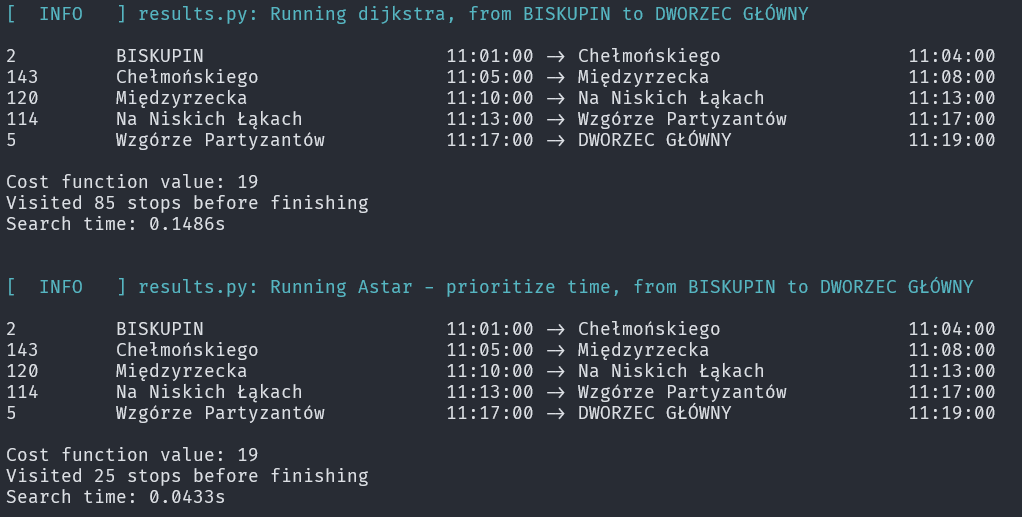
\includegraphics[width=0.8\textwidth]{2024-04-07-12-54-53.png} 
  \end{figure}
  Jak widać, Dijkstra oraz A* znalazły tą samą trasę, która wymaga wielu 
  przesiadek, jednak pozwala dotrzeć na miejsce w krótkim czasie.
  Czas wykonania A* był prawie 4 razy mniejszy niż Dijkstra.
  
  \item Trasa KRZYKI -> Bielany Wrocławskie - Kościół o 13:15
  \begin{figure}[H]
    \centering
    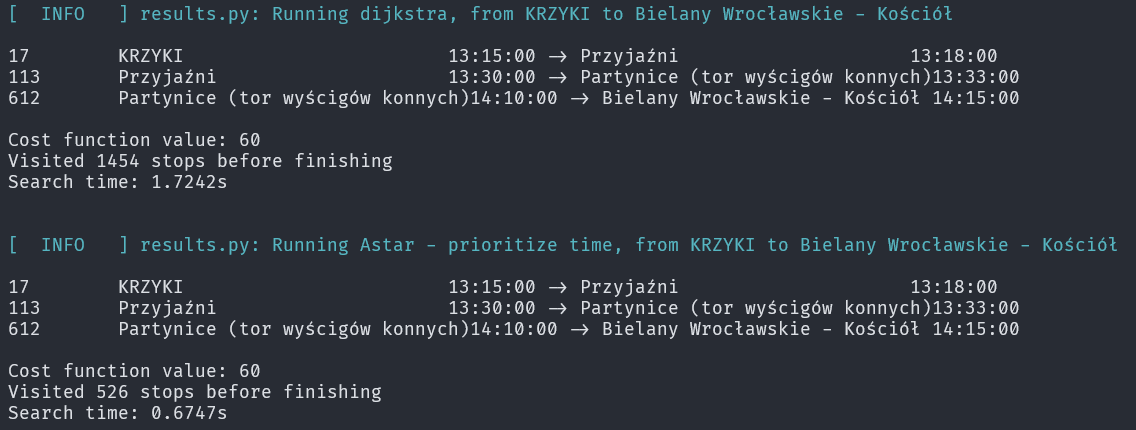
\includegraphics[width=0.8\textwidth]{2024-04-07-12-58-54.png} 
  \end{figure}
  Ponownie, oba algorytmy znalazły tą samą trasę.
  Znalezienie trasy zajęło A* około 3 razy mniej czasu.
 
  \item Trasa KMINKOWE -> DWORZEC AUTOBUSOWY o 00:00
  \begin{figure}[H]
    \centering
    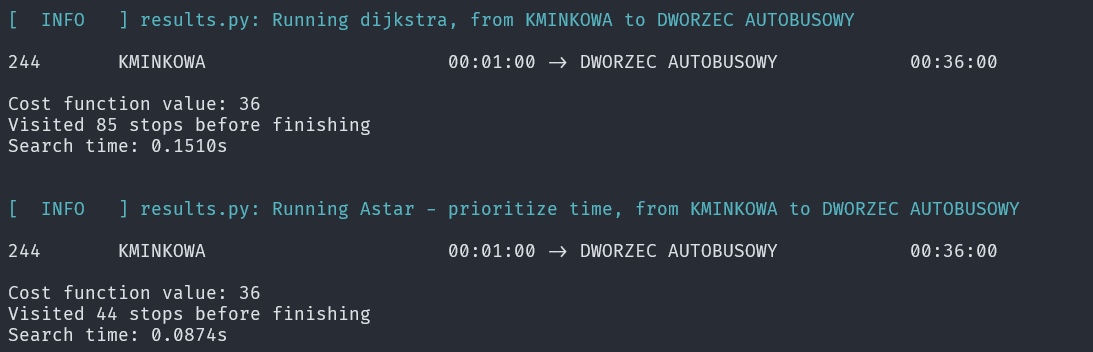
\includegraphics[width=0.8\textwidth]{2024-04-08-06-14-05.png} 
  \end{figure}
  Ponownie, oba algorytmy znalazły tą samą trasę.
  Znalezienie trasy zajęło A* około 3 razy mniej czasu.

\end{itemize}


\subsubsection{Kryterium przesiadek}


\begin{itemize}
  \item Trasa BISKUPIN -> DWORZEC GŁÓWNY o 11:00
  \begin{figure}[H]
    \centering
    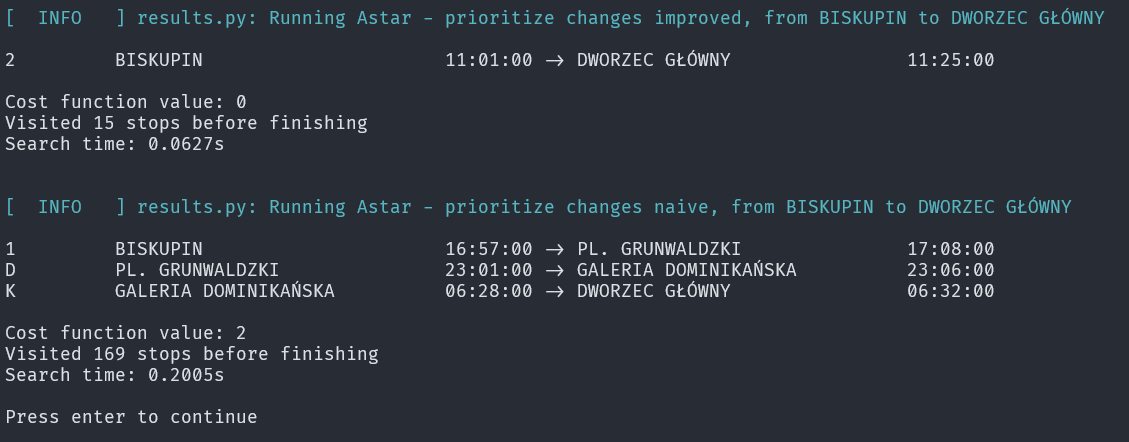
\includegraphics[width=0.8\textwidth]{2024-04-07-13-00-26.png} 
  \end{figure}
  Różnica pomiędzy naiwną wersją a zoptymalizowaną jest ogromna.
  Zoptymalizowana wersja znalazła trasę bez przesiadek.
  Naiwna implementacja wymagała aż 2 przesiadek,
  a dodatkowo nie bierze pod uwagę czasu podróży.

  \item Trasa KRZYKI -> Bielany Wrocławskie - Kościół o 13:15
  \begin{figure}[H]
    \centering
    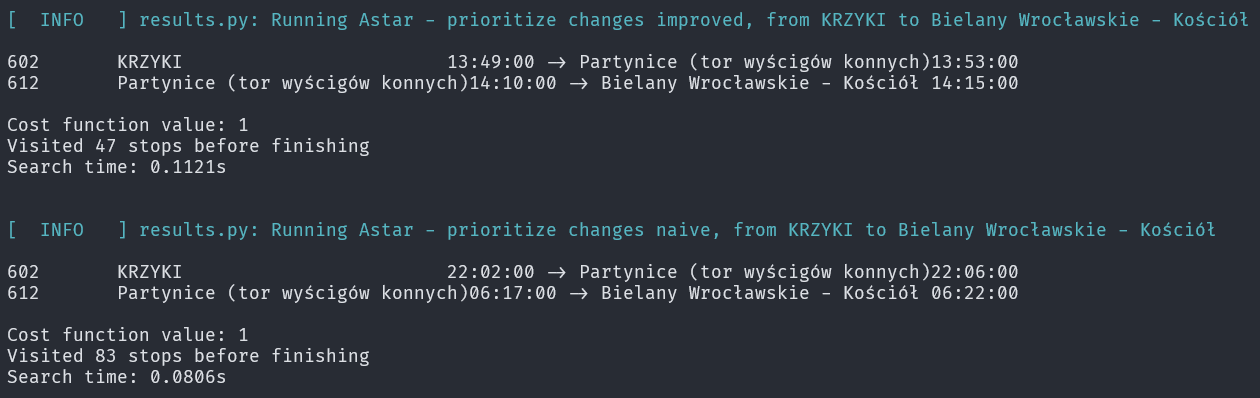
\includegraphics[width=0.8\textwidth]{2024-04-07-13-02-12.png} 
  \end{figure}
  W tym wypadku oba algorytmy wymagają 1 przesiadki, jednak zoptymalizowana wersja
  pozwala na szybsze dotarcie do celu.

  \item Trasa Katedra -> Zaolziańska o 22:00
  \begin{figure}[H]
    \centering
    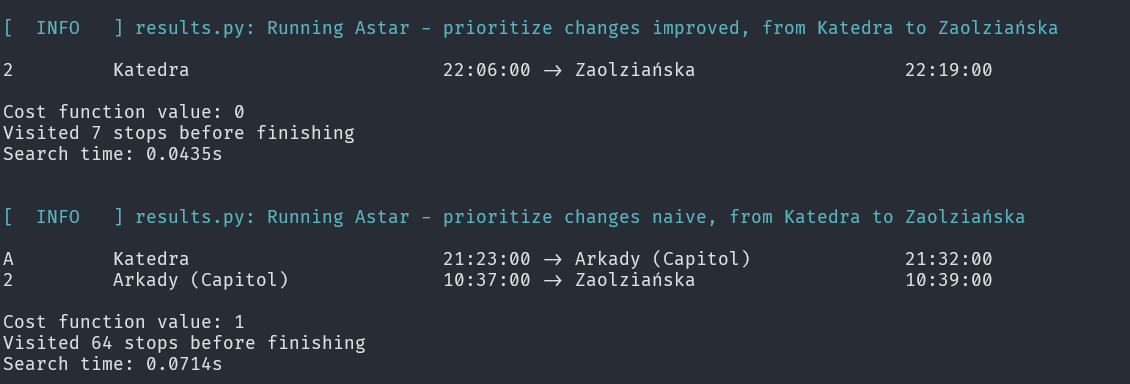
\includegraphics[width=0.8\textwidth]{2024-04-08-06-11-42.png} 
  \end{figure}
  Można także zaobserwoać, że pomimo bardziej skomplikowanych obliczeń (sortowanie tras),
  ulepszona wersja dzęsto działa szybciej niż naiwna (odwiedza mniej przystanków przed znalezieniem trasy).

\end{itemize}


\section{Zadanie 2}
\subsection{Algorytm Tabu Search, bez ograniczenia tablicy T}
\subsubsection{Opis}

Algorytm działa poprzez przeszukiwanie przestrzeni rozwiązań w celu znalezienia
najlepszego rozwiązania. Rozwiązaniem jest tutaj permutacja kolejności przystanków,
która pozwoli zminimalizować czas podróży lub liczbę przesiadek. 
Generowane jest rozwiązanie początkowe (jest to ewaluacja kolejnośći przystanków 
otrzymanej w parametrze), a następnie przeszukiwana jest przestrzeń rozwiązań
sąsiednich, poprzez generowanie sąsiedztwa za pomocą zamiany dwóch przystanków.
Rozwiązania sąsiedznie są oceniane, a następnie wybierane jest najlepsze z nich,
które nie należy do listy tabu, a następnie dodawane do listy tabu.
Cały cykl powtarza się aż do spełnienia warunku stopu, który 
w tym wypadku jest liczbą iteracji. W celu wyznaczenia trasy pomiędzy poszczególnymi
przystankami używany jest algorytm A*, używający jako heurestyki odległość haversine,
ponieważ spisywał się on najlepiej.

\subsubsection{Kod}

\begin{itemize}
    \item Główny algorytm
\begin{lstlisting}
def tabu_search(
    graph: Graph,
    start: Stop,
    to_visit: list[Stop],
    departure_min: int,
    search_function: Callable,
    max_iterations: int,
) -> TabuSearchResult:
    best_solution: TabuSearchResult = create_path_between_stops(
        graph, [start] + to_visit + [start], departure_min, search_function
    )
    current_solution = best_solution

    tabu_list: list[TabuSearchResult] = []

    for _ in range(max_iterations):
        neighbors = get_neighbors(current_solution.to_visit)
        best_neighbor_solution = None
        best_cost = float("inf")

        for neighbor in neighbors:
            if neighbor not in tabu_list:
                neighbor_solution = create_path_between_stops(
                    graph, neighbor, departure_min, search_function
                )

                if neighbor_solution.total_cost < best_cost:
                    best_neighbor_solution = neighbor_solution
                    best_cost = neighbor_solution.total_cost

        if best_neighbor_solution is None:
            break

        current_solution = best_neighbor_solution
        tabu_list.append(best_neighbor_solution)

        if best_neighbor_solution.total_cost < best_solution.total_cost:
            best_solution = best_neighbor_solution

    return best_solution
\end{lstlisting}

    \item Funkcja generująca sąsiedztwo
\begin{lstlisting}
def get_neighbors(current_solution: list[Stop]) -> list[list[Stop]]:
    n = len(current_solution)
    neighbors = []

    for i in range(1, n - 1):
        for j in range(i + 1, min(i + 3, n - 1)):
            neighbor = current_solution[:]
            neighbor[i], neighbor[j] = neighbor[j], neighbor[i]
            neighbors.append(neighbor)

    return neighbors
\end{lstlisting}
    Funkcja generująca sąsiedztwo poprzez zamianę dwóch przystanków.
    Funkcja omija pierwszy i ostatni przystanek, ponieważ jest to przystanek początkowy.
    W celu ograniczenia liczby generowanych sąsiadów, wewnętrzna pętla jest ograniczona
    do 3 przystanków od aktualnego przystanku.

    \item Funkcja tworząca ścieżkę pomiędzy przystankami
\begin{lstlisting}
def create_path_between_stops(
    graph, to_visit: list[Stop], departure_min: int, search_function: Callable
) -> TabuSearchResult:
    came_from: list[SearchResult] = []
    total_cost: float = 0
    current_min: int = departure_min

    for i in range(len(to_visit) - 1):
        start_stop: Stop = to_visit[i]
        end_stop: Stop = to_visit[i + 1]
        result: SearchResult = search_function(graph, start_stop, end_stop, current_min)
        arrival_min: int = result.came_from[end_stop].arrival_min
        total_cost += result.costs[end_stop]
        came_from.append(result)
        current_min = arrival_min

    return TabuSearchResult(came_from, to_visit, total_cost)
\end{lstlisting}
    Funkcja ta tworzy ścieżkę pomiędzy przystankami, używając podanego algorytmu.
    Zwraca ona strukturę TabuSearchResult, która zawiera informacje o kosztach, poprzednikach, przyjętej kolejności
    przystanków oraz całkowitym koszcie podróży.
\end{itemize}


\subsubsection{Przykładowe działanie}


\begin{itemize}
    \item Trasa BISKUPIN -> ['DWORZEC GŁÓWNY', 'Ogród Botaniczny', 'Dubois', 'PL. GRUNWALDZKI'] -> BISKUPIN 0 8:00
  \begin{figure}[H]
    \centering
    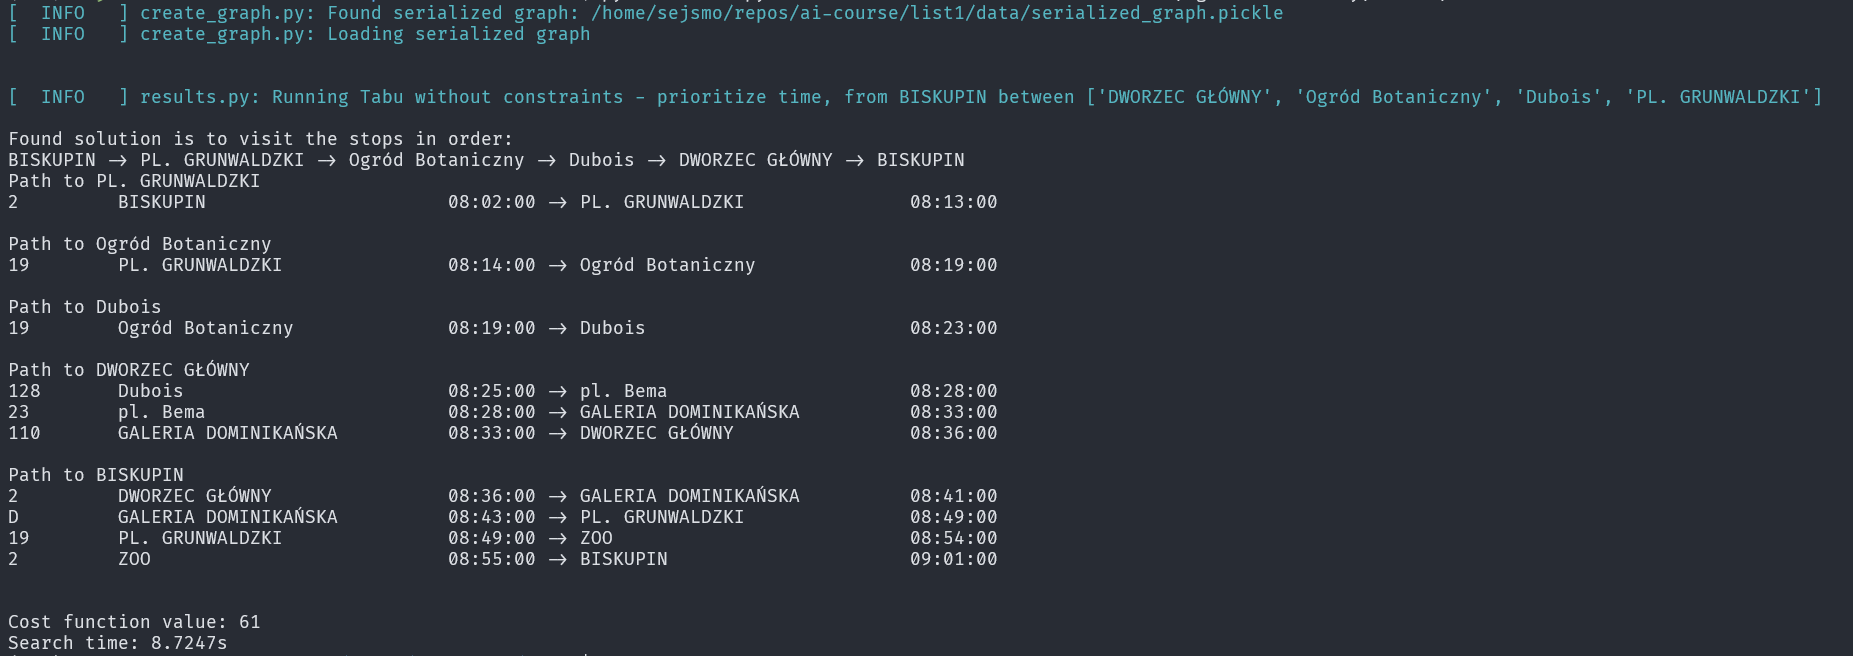
\includegraphics[width=0.9\textwidth]{2024-04-08-07-36-38.png} 
  \end{figure}
  Jak widać dla 4 przysstanków czas przeszukiwania wyniósło około 8s.
  Otrzymany wynik wydaje się prawidłowy - przystanki są odwiedzane w kolejności,
  która pozwala na zminimalizowanie czasu podróży.


    \item Trasa GALERIA DOMINIKAŃSKA -> ['Paprotna', 'Wyszyńskiego', 'KMINKOWA'] ->GALERIA DOMINIKAŃSKA 
  \begin{figure}[H]
    \centering
    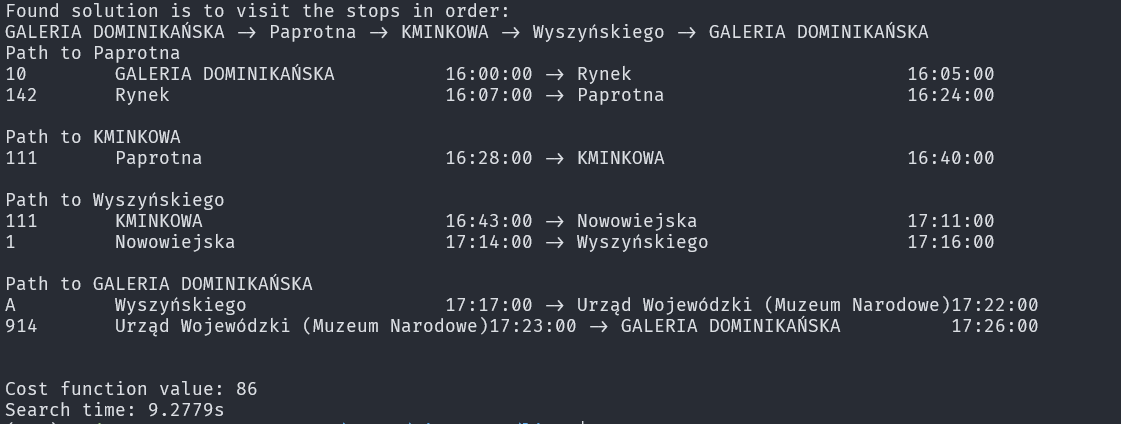
\includegraphics[width=0.9\textwidth]{2024-04-08-07-48-31.png} 
  \end{figure}
\end{itemize}


\subsection{Dobór tługości listy T}
    \subsubsection{Opis}
    W tym kroku, dodano do algorytmu parametr, który pozwala na ograniczenie długości listy tabu.
    Rozwiązanie takie, pomaga zredukować użycie pamięci oraz uniknąć zatrzymania w pewnym obszarze poszukiwań.
    Usunięcie starszych elementów z listy daje możliwość ponownego przeszukania obszaru, który był wcześniej
    na liście tabu. 

    \subsubsection{Kod}
\begin{lstlisting}
# def tabu_search(
#     graph: Graph,
#     start: Stop,
#     to_visit: list[Stop],
#     departure_min: int,
#     search_function: Callable,
#     max_iterations: int,
    tabu_list_size: Optional[int] = None,
# ) -> TabuSearchResult:
#     best_solution: TabuSearchResult = create_path_between_stops(
#         graph, [start] + to_visit + [start], departure_min, search_function
#     )
#     current_solution = best_solution
# 
#     tabu_list: list[TabuSearchResult] = []
# 
#     for _ in range(max_iterations):
#         neighbors = get_neighbors(current_solution.to_visit)
#         best_neighbor_solution = None
#         best_cost = float("inf")
# 
#         for neighbor in neighbors:
#             if neighbor not in tabu_list:
#                 neighbor_solution = create_path_between_stops(
#                     graph, neighbor, departure_min, search_function
#                 )
# 
#                 if neighbor_solution.total_cost < best_cost:
#                     best_neighbor_solution = neighbor_solution
#                     best_cost = neighbor_solution.total_cost
# 
#         if best_neighbor_solution is None:
#             break
# 
#         current_solution = best_neighbor_solution
#         tabu_list.append(best_neighbor_solution)
        if tabu_list_size and len(tabu_list) > tabu_list_size:
            tabu_list.pop(0)
# 
#         if best_neighbor_solution.total_cost < best_solution.total_cost:
#             best_solution = best_neighbor_solution
# 
#     return best_solution
\end{lstlisting}
Dodano parametr tabu\_list\_size, który pozwala na ograniczenie długości listy tabu.
W przypadku przekroczenia tej długości, usuwany jest najstarszy element z listy(czyli element o indeksie 0, 
ponieważ dodawanie następuje na koniec listy).



  






\end{document}